% DOCUMENT SETUP
\documentclass[letterpaper,11pt]{article}
\hyphenpenalty=8000
\textwidth=125mm
\textheight=200mm
\usepackage[top=3cm, bottom=3cm, inner=3cm, outer=3cm, includehead]{geometry}
\usepackage{fancyhdr}
\setlength{\headheight}{13.6pt} % Fix for fancyhdr warning
\addtolength{\topmargin}{-1.6pt} % Optional: further fix as suggested
\pagestyle{fancy}
\fancyhead{}
\fancyfoot{}
\raggedbottom
\usepackage{xurl}
\usepackage{graphicx}
\usepackage{xcolor}
\usepackage{amssymb}
\usepackage{mathtools}
\usepackage{alltt}
\usepackage{amsmath}
\usepackage[pdftex, hidelinks]{hyperref}
\urlstyle{same}
\usepackage[T1]{fontenc}
\usepackage[utf8]{inputenc}
\usepackage{lmodern}
\usepackage{csquotes}
\usepackage[notes, backend=biber]{biblatex-chicago}
\pagenumbering{arabic}
\setcounter{page}{1}
\graphicspath{{./imgs/}}
\usepackage[english]{babel}
\usepackage{multirow}
\usepackage{tabularx}
\usepackage{fancyvrb}
\usepackage{caption}
%\usepackage[french]{babel}
%\usepackage[spanish]{babel}

% AUTHOR AND TITLE
\begin{document}
\fancyhead[RO]{ELEC 475 Lab 2, Alistair Barfoot and Luke Barry\ \ \ \ \thepage}
\begin{center}
  \LARGE
  \textbf{ELEC 475 Lab 2, Alistair Barfoot and Luke Barry}\\[12pt]
  \normalsize
\end{center}
\tableofcontents

\newpage

\section{Network Architecture}
SnoutNet is a Convolutional Neural Network designed for regressing the (x,y) coordinates of an animal's nose from a RGB image. It takes an input image of 227x227x3 and outputs a 2D coordinate vector. It is comprised of three convolutional blocks each followed by a ReLU activation and a Max Pooling layer, then three fully connected (FC) layers.

\begin{table}[h]
  \centering
  % \resizebox{\linewidth}{!}{
  \begin{tabularx}{\linewidth}{|c|c|c|X|}
    \hline
    \textbf{Layer}    & \textbf{Input Shape} & \textbf{Output Size} & \textbf{Parameters}                                                                                      \\
    \hline
    \textbf{Conv1}    & 227x227x3            & 114x114x64           & \verb+in_channels=3+, \verb+out_channels=64+, \verb+kernel_size=3+, \verb+stride=2+, \verb+padding=1+    \\
    \hline
    \textbf{ReLU1}    & 114x114x64           & 114x114x64           &                                                                                                          \\
    \hline
    \textbf{MaxPool1} & 114x114x64           & 57x57x64             & \verb+kernel_size=3+, \verb+stride=2+, \verb+padding=1+                                                  \\
    \hline
    \textbf{Conv2}    & 57x57x64             & 29x29x128            & \verb+in_channels=64+, \verb+out_channels=128+, \verb+kernel_size=3+, \verb+stride=2+, \verb+padding=1+  \\
    \hline
    \textbf{ReLU2}    & 29x29x128            & 29x29x128            &                                                                                                          \\
    \hline
    \textbf{MaxPool2} & 29x29x128            & 15x15x128            & \verb+kernel_size=3+, \verb+stride=2+, \verb+padding=1+                                                  \\
    \hline
    \textbf{Conv3}    & 15x15x128            & 8x8x256              & \verb+in_channels=128+, \verb+out_channels=256+, \verb+kernel_size=3+, \verb+stride=2+, \verb+padding=1+ \\
    \hline
    \textbf{ReLU3}    & 8x8x256              & 8x8x256              &                                                                                                          \\
    \hline
    \textbf{MaxPool3} & 8x8x256              & 4x4x256              & \verb+kernel_size=3+, \verb+stride=2+, \verb+padding=1+                                                  \\
    \hline
    \textbf{FC1}      & 4x4x256(4096)        & 1024                 &                                                                                                          \\
    \hline
    \textbf{ReLU4}    & 1024                 & 1024                 &                                                                                                          \\
    \hline
    \textbf{FC2}      & 1024                 & 1024                 &                                                                                                          \\
    \hline
    \textbf{ReLU5}    & 1024                 & 1024                 &                                                                                                          \\
    \hline
    \textbf{FC3}      & 1024                 & 2 (u,v)              &                                                                                                          \\
    \hline
  \end{tabularx}
  % }
\end{table}

\section{DataLoader and Dataset}
The images and labels are loaded through a custom pytorch dataset class called CustomDataset, which reads the annotation file train-noses.txt containing image file names and their corresponding coordinates to their noses. For each entry the dataset loads the image and converts it to an RGB format and parses the coordinate string to numerical values. Images are resized to 227x227 pixels and the transformed nose coordinates are returned as a vector.\\
\\
A factcheck was performed by creating a small test script that loads a sample and prints the shapes and values. Throughout each train an \verb+example_debug.png+ image will appear one in every thousand images with the image and its corresponding snout vector. This ensures that the dataset is loading correctly each time with the augmentation applied.

\section{Hyperparameters}
The SnoutNet model was trained for 50 epochs with a batch size of 32 using the Adam optimizer and Kaiming Normal weight initialization. The learning rate scheduler is applied to monitor validation loss and reduces the learning rate by a factor of 2 if no improvement has been observed in 3 consecutive epochs. The learning rate was set to $3\times10^{-4}$ and a weight decay of $3\times10^{-6}$. \\
\\
The loss function used was the Mean Squared Error (MSE) loss. Early stopping is also implemented if no validation loss improvement has been observed for 5 epochs. In the case of early stopping, the model weights are reverted to the best observed validation loss.

\section{Augmentation}
Data augmentation was optionally applied to the training. A horizontal flip to simulate mirrored images was applied as well as a random rotation of $\pm10 ^{\circ}$ to provide rotational variance. For both horizontal flip and a random rotation, the label for the nose vector needed to be adjusted, since the images position within the frame changed the snout of each animal would have changed in position too.\\
\\
The horizontal flip occured with a probability of 0.1, and the random rotation was applied with a probability of 1.

\newpage
\section{Results}
The training was conducted on a NVIDIA RTX 3060 Super laptop edition. To calculate the distance from ground truth for testing, the distances were adjusted to account for the resizing of the images to 227x227 pixels and rounded to the nearest integer.\\
\\
The training results for each model and augmentation strategy are summarized in Table \ref{tab:training_results}, while the error statistics are presented in Table \ref{tab:localization_error_stats}.

\begin{table}[h!]
  \centering
  \resizebox{\linewidth}{!}{
    \begin{tabular}{|c|c|c|c|c|c|}
      \hline
      \textbf{Model}              & \textbf{Augmentation} & \textbf{Epochs} & \textbf{Train Loss} & \textbf{Test Loss} & \textbf{Time Elapsed (h:mm)} \\
      \hline
      \multirow{4}{*}{SnoutNet}   & None                  & 26              & 213                 & 398                & 0:13                         \\
      \cline{2-6}                 & Flip                  & 26              & 347                 & 541                & 0:14                         \\
      \cline{2-6}                 & Rotate                & 33              & 291                 & 455                & 0:18                         \\
      \cline{2-6}                 & Flip / Rotate         & 50              & 395                 & 427                & 0:27                         \\
      \hline
      \multirow{4}{*}{SnoutNet-A} & None                  & 14              & 87                  & 168                & 0:10                         \\
      \cline{2-6}                 & Flip                  & 16              & 72                  & 182                & 0:11                         \\
      \cline{2-6}                 & Rotate                & 34              & 55                  & 119                & 0:24                         \\
      \cline{2-6}                 & Flip/Rotate           & 43              & 51                  & 103                & 0:31                         \\
      \hline
      \multirow{4}{*}{SnoutNet-V} & None                  & 6               & 94                  & 147                & 0:46                         \\
      \cline{2-6}                 & Flip                  & 9               & 118                 & 123                & 1:09                         \\
      \cline{2-6}                 & Rotate                & 20              & 35                  & 87                 & 2:34                         \\
      \cline{2-6}                 & Flip/Rotate           & 14              & 131                 & 129                & 1:48                         \\
      \hline
    \end{tabular}
  }
  \caption{Training results for each model and augmentation strategy.}
  \label{tab:training_results}
\end{table}

% \newpage
\begin{table}[h!]
  \centering
  \resizebox{\linewidth}{!}{
    \begin{tabular}{|c|c|c|c|c|c|c|c|c|c|c|c|c|c|}
      \hline
      \multirow{2}{*}{Model}      & \multirow{2}{*}{Augmentation} & \multicolumn{4}{|c|}{Localization Error} & \multicolumn{4}{|c|}{Localization Error (4 Worst)} & \multicolumn{4}{|c|}{Localization Error (4 Best)}                                                               \\
      \cline{3-14}                &                               & min                                      & max                                                & mean                                              & stdev & min & max & mean & stdev & min & max & mean & stdev \\
      \hline
      \multirow{4}{*}{SnoutNet}   & None                          & 1                                        & 145                                                & 26                                                & 19.3  & 106 & 145 & 122  & 16.4  & 1   & 2   & 1    & 0.4   \\
      \cline{2-14}
                                  & Flip                          & 1                                        & 132                                                & 26                                                & 19.2  & 109 & 132 & 119  & 9.3   & 1   & 2   & 1    & 0.4   \\
      \cline{2-14}
                                  & Rotate                        & 1                                        & 171                                                & 24                                                & 19.5  & 113 & 171 & 136  & 22.1  & 1   & 1   & 1    & 0.2   \\
      \cline{2-14}
                                  & Flip/Rotate                   & 0                                        & 140                                                & 23                                                & 18.1  & 103 & 140 & 123  & 13.7  & 0   & 2   & 1    & 0.6   \\
      \hline
      \multirow{4}{*}{SnoutNet-A} & None                          & 0                                        & 117                                                & 14                                                & 13.4  & 82  & 117 & 94   & 13.5  & 0   & 1   & 1    & 0.1   \\
      \cline{2-14}
                                  & Flip                          & 0                                        & 99                                                 & 13                                                & 12.5  & 73  & 99  & 88   & 10.0  & 0   & 1   & 1    & 0.1   \\
      \cline{2-14}
                                  & Rotate                        & 0                                        & 111                                                & 10                                                & 12.7  & 71  & 111 & 93   & 14.5  & 0   & 1   & 0    & 0.2   \\
      \cline{2-14}
                                  & Flip/Rotate                   & 0                                        & 116                                                & 10                                                & 11.1  & 68  & 116 & 85   & 18.4  & 0   & 0   & 0    & 0.2   \\
      \hline
      \multirow{4}{*}{SnoutNet-V} & None                          & 0                                        & 107                                                & 10                                                & 13.3  & 84  & 107 & 96   & 9.7   & 0   & 0   & 0    & 0.2   \\
      \cline{2-14}
                                  & Flip                          & 0                                        & 88                                                 & 10                                                & 9.3   & 71  & 88  & 82   & 6.3   & 0   & 1   & 1    & 0.2   \\
      \cline{2-14}
                                  & Rotate                        & 1                                        & 120                                                & 9                                                 & 10.0  & 80  & 120 & 93   & 15.7  & 1   & 1   & 1    & 0.1   \\
      \cline{2-14}
                                  & Flip/Rotate                   & 0                                        & 110                                                & 9                                                 & 11.1  & 84  & 110 & 94   & 9.8   & 0   & 1   & 0    & 0.1   \\
      \hline
      \multirow{4}{*}{Ensemble}   & None                          & 0                                        & 115                                                & 13                                                & 13.2  & 85  & 115 & 95   & 11.9  & 0   & 1   & 0    & 0.3   \\
      \cline{2-14}
                                  & Flip                          & 0                                        & 93                                                 & 13                                                & 11.8  & 72  & 93  & 86   & 8.2   & 0   & 1   & 0    & 0.3   \\
      \cline{2-14}
                                  & Rotate                        & 0                                        & 110                                                & 12                                                & 12.2  & 87  & 110 & 97   & 8.8   & 0   & 1   & 1    & 0.1   \\
      \cline{2-14}
                                  & Flip/Rotate                   & 0                                        & 93                                                 & 13                                                & 11.8  & 72  & 93  & 86   & 8.2   & 0   & 1   & 0    & 0.3   \\
      \hline

      \hline
    \end{tabular}%
  }
  \captionof{table}{Localization error statistics for each model and augmentation strategy.}
  \label{tab:localization_error_stats}
\end{table}

\newpage
\noindent
Tables \ref{tab:snoutpics}, \ref{tab:alexpics}, and \ref{tab:vggpics} show randomly selected example images from the test set with predicted snout positions from each of the three model architectures when trained with both augmentations (flip and rotate). The green circle represents the predicted snout position, while the blue circle represents the ground truth snout position.

\begin{table}[h!]
  \centering
  \begin{tabular}{ll}
    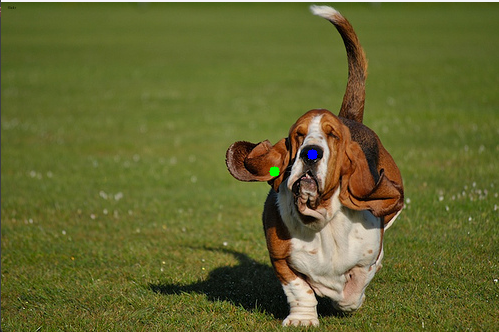
\includegraphics[width=0.3\linewidth]{pics/Snoutnet1.png} & 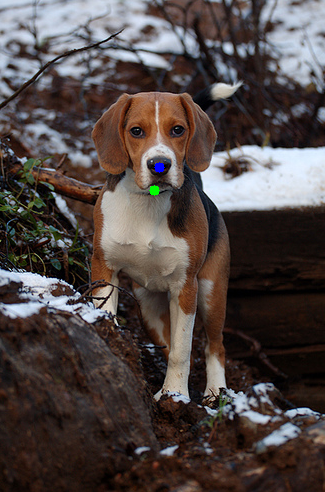
\includegraphics[width=0.15\linewidth]{pics/snoutnet2.png} \\
    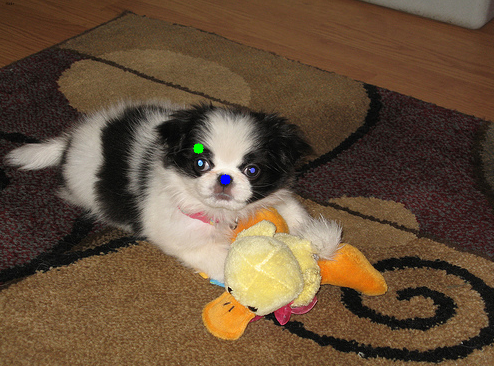
\includegraphics[width=0.3\linewidth]{pics/snoutnet3.png} & 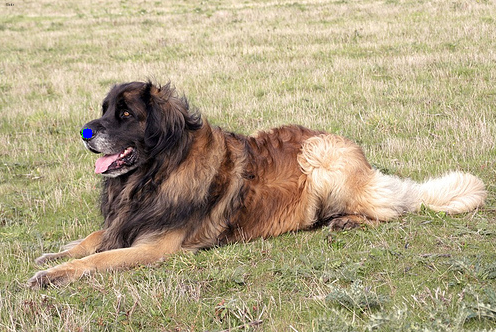
\includegraphics[width=0.3\linewidth]{pics/snoutnet4.png}  \\
  \end{tabular}
  \caption{Example images from SnoutNet base model with both augmentations}
  \label{tab:snoutpics}
\end{table}

\begin{table}[h!]
  \centering
  \begin{tabular}{ll}
    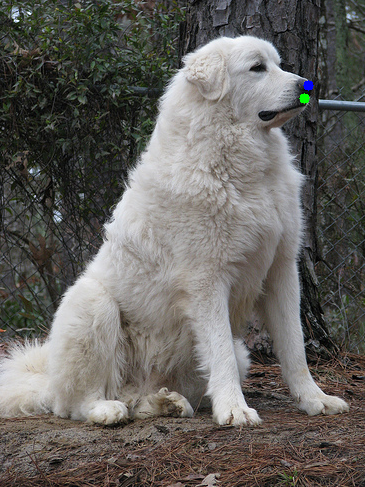
\includegraphics[width=0.2\linewidth]{pics/alex1.png} & 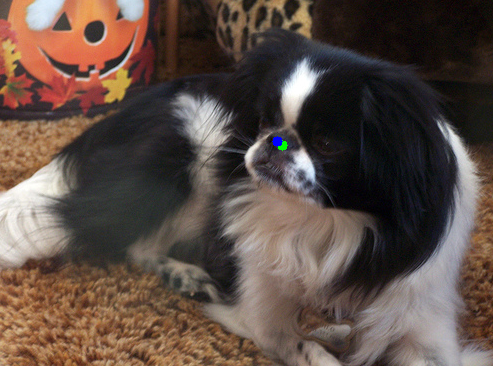
\includegraphics[width=0.35\linewidth]{pics/alex2.png}  \\
    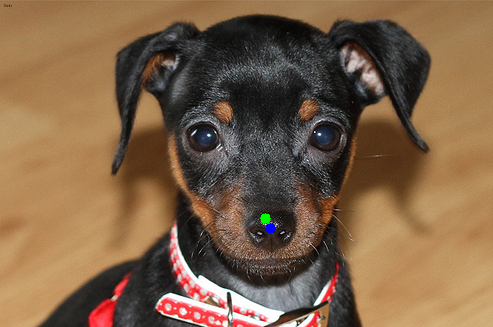
\includegraphics[width=0.3\linewidth]{pics/alex3.png} & 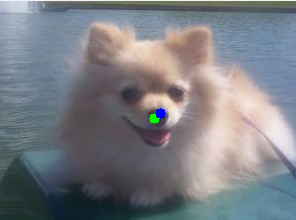
\includegraphics[width=0.275\linewidth]{pics/alex4.png} \\
  \end{tabular}
  \caption{Example images from SnoutNet-A model with both augmentations}
  \label{tab:alexpics}
\end{table}

\begin{table}[h!]
  \centering
  \begin{tabular}{ll}
    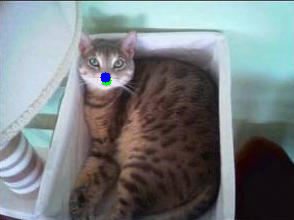
\includegraphics[width=0.3\linewidth]{pics/Vggnet1.png} & 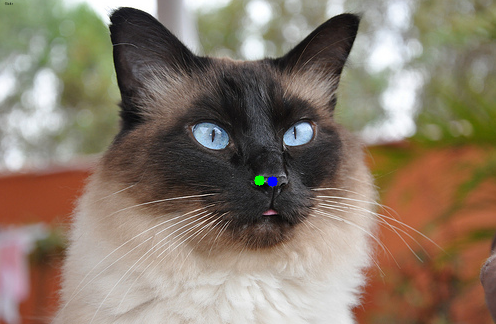
\includegraphics[width=0.3\linewidth]{pics/vgg2.png} \\
    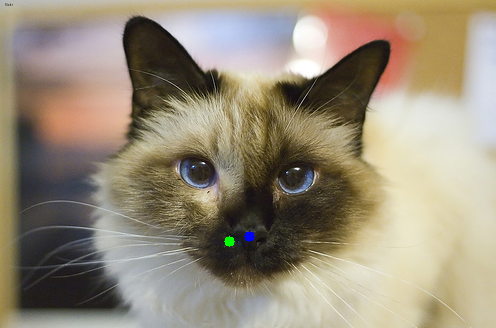
\includegraphics[width=0.3\linewidth]{pics/vgg3.png}    & 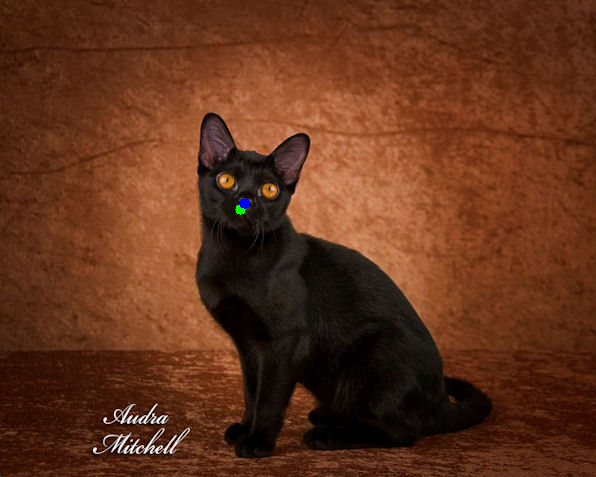
\includegraphics[width=0.3\linewidth]{pics/vgg4.png} \\
  \end{tabular}
  \caption{Example images from SnoutNet-V model with both augmentations}
  \label{tab:vggpics}
\end{table}

\newpage
\newpage
\newpage

\section{Performance}
% Discuss the performance of your system. How well did it perform? Was the performance as expected? Discuss which (if any) of the augmentation methods were beneficial. What challenges did you experience, and how did you overcome them?
Overall, the model performed well in identifying the snout position of the animals in the images. The best performing (non-ensemble) model was SnoutNet-V trained with rotation augmentation, achieving a mean localization error of 9 pixels with a standard deviation of 10.0 pixels. This model achieved a test loss of 87 while training and reached 20 epochs before early stopping.\\
\\
In general, the flip augmentation did not significantly improve performance, and in the case of SnoutNet-V, it actually led to a slight decrease in performance when going from rotation only to flip/rotate. \\
\\
The SnoutNet architecture was the worst-performing model overall when compared to the SnoutNet-A and SnoutNet-V variants. This was expected, as the latter two models have much more parameters and more advanced techniques such as dropout. The SnoutNet-A model performed better than the base model, but just slightly worse than SnoutNet-V despite the significant different in model size and training time. \\

\newpage
\section{Ensemble Approach}
% Describe how your ensemble approach combined the infromation from the three models. Discuss how this impacted performance.
The ensemble approach combined the predictions from each of the three models by asking each model to predict the snout position for a given image, then averaging the (u,v) coordinates from each model to arrive at a final prediction. \\
\\
Overall, the ensemble approach had a negative impact on the performance of the model. All of the SnoutNet-V and most of the SnoutNet-A individual models outperformed the ensemble in terms of mean localization error. This is due to the fact that the base model SnoutNet performed poorly, which drags down to overall performance when averaging the predictions. In the future, to improve on the ensemble approach, a weighted average could be used where better-performing models have a higher weight in the final prediction. This can be tuned using trial-and-error on the validation set to find the optimal weights for each model.

\section{LLM Usage}
% Share the link to your conversation with LLM of your choice (e.g., ChatGPT, Claude, etc.). How did you make sure that code or concepts generated by LLM were not hallucinations?
\textcolor{blue}{\textbf{\href{https://github.com/copilot/share/88025032-03a4-8871-b803-a44664ab6910}{Link to LLM Conversation}}}\\
\\
For this lab, GitHub Copilot was used to assist in generating the structure of the SnoutNet dataset and DataLoader classes. However, the code generated by the LLM was not just copied and ran in the project. Instead, each line of the code generated by the LLM was carefully reviewed and tested to ensure that it functioned as intended. \\
\\
Debugging files and lines were added at every step of the process to ensure that each part was functioning correctly and as predicted. In the final version of the lab, much of the code generated by the LLM has been modified or removed entirely as it was not taken just at face value.\\
\\
Claude Sonnet 4 was used for the creation of the README.md file in the base repository. It was prompted to create a well-structured and informative README with the context of the lab project provided.


\end{document}